\documentclass{article}
\usepackage[T1]{fontenc}
\usepackage[utf8]{inputenc}

\usepackage{cmbright}
\usepackage[T1]{fontenc}

\usepackage{multicol}

\usepackage{amsmath}
\usepackage{amsfonts}
\usepackage{amssymb}
\usepackage{tikz}
\usepackage{graphicx}
\graphicspath{  {./images/} }
\setlength{\parindent}{0pt}
\usepackage{changepage}
\usepackage{verbatim}
\usepackage{physics}
\usepackage{derivative}
\usepackage{bm}
\usepackage[colorlinks=true, linkcolor=blue, urlcolor=blue, citecolor=blue, anchorcolor=blue]{hyperref}

\addtolength{\oddsidemargin}{-.25in}
\addtolength{\textwidth}{0.5in}

\makeatletter
\newcommand*\bigcdot{\mathpalette\bigcdot@{.5}}
\newcommand*\bigcdot@[2]{\mathbin{\vcenter{\hbox{\scalebox{#2}{$\m@th#1\bullet$}}}}}
\makeatother

\DeclareMathOperator{\di}{d\!}
\newcommand*\Eval[3]{\left.#1\right\rvert_{#2}^{#3}}

\newcommand{\uvec}[1]{\boldsymbol{\hat{\textbf{#1}}}}
\newcommand{\vr}[1]{\textbf{#1}}

\newcommand{\thus}[0]{\; \; \longrightarrow \; \;}

\newcommand{\lag}{\mathcal{L}}
\newcommand{\ham}{\mathcal{H}}

\title{Black Hole Spin Simulations}
\author{Ryan Liu}
\date{Last updated: June 1, 2021}

\begin{document}

\maketitle

\section{Resources Used}

\section{Notes}

\section{Results}

\begin{figure}[!htb]
    \center{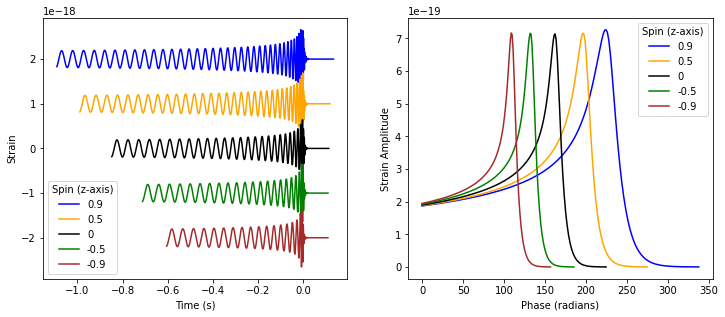
\includegraphics[width=\textwidth]{SNR23.png}}
    \caption{\label{fig:label} Expectation SNR of a 30 $M_\odot$ black hole merger at aLIGO design sensitivity; the distance resolution is $0.05$ Mpc}
\end{figure}

\begin{figure}[!htb]
    \center{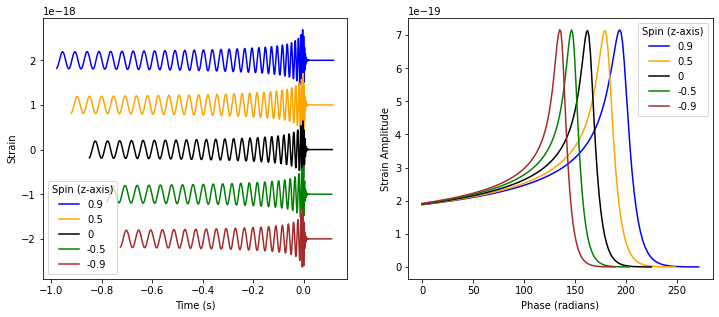
\includegraphics[width=\textwidth]{SNR24.png}}
    \caption{\label{fig:label} Expectation SNR of a 30 $M_\odot$ black hole merger at aLIGO design sensitivity; the distance resolution is $0.05$ Mpc}
\end{figure}

\begin{figure}[!htb]
    \center{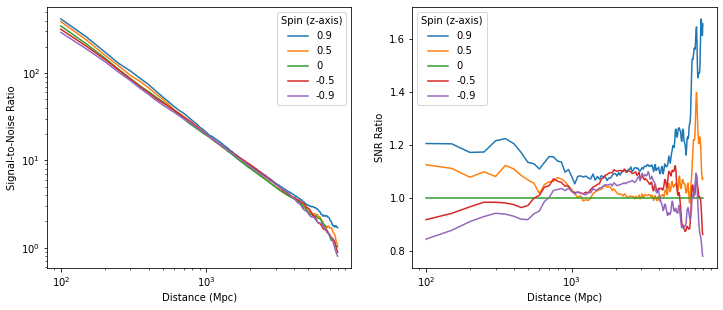
\includegraphics[width=\textwidth]{SNR25.png}}
    \caption{\label{fig:label} Expectation SNR of a 30 $M_\odot$ black hole merger at aLIGO design sensitivity; the distance resolution is $0.05$ Mpc}
\end{figure}





\end{document}